\section{Introduction}

Recommendation systems are a vital component of the modern Web.  They
help readers effectively navigate otherwise unwieldy archives of
information and help websites direct users to items---movies,
articles, songs, apps---that they will like.  A recommendation system
is built from user behavior data, historical data about which items
each user has consumed.  First, a statistical machine learning
algorithm is used to uncover behavioral patterns that reveal the
various types of users and the items they tend to like.  Then, the
system exploits these discovered patterns to recommend future items to
its users.

As an example, Figure 1 illustrates movie recommendation for a user
$U$ from the MovieLens data set~\cite{Herlocker:1999}.  This data set
is a large sparse matrix where rows are people and columns are movies.
Each entry of the matrix (indexed by a user and a movie) contains the
rating that the user gave to the movie, or a zero if she has not seen
it. The list of movies at the top of the
\myfig{movielens-illustration} shows that user $U$ enjoys various
types of drama movies (such as the war drama ``Breaker Morant'' and
the romantic drama ``Leaving Las Vegas''). Of course, she has only
seen a handful of the available movies, and the goal of a
recommendation system is to suggest other movies.  The list of movies
at the bottom of the figure was suggested by our algorithm. It
includes other war drama movies (such as "Apocalypse Now") and other
romantic drama (such as "Breakfast at Tiffany's").  In this paper, we
develop a new algorithm for building recommendation systems that is
both more efficient and performs better than the existing
state-of-the-art.

%% \begin{figure*}[th]
%% \centering
%% \caption{The top 5 movies in each of the top 4 components of the user
%%   $U$ illustrated in Fig~\ref{fig:movielens-illustration}.}
%% \vspace{0.1cm}
%% \small
%% \begin{tabular}{c}
%% \toprule
%% \bf{``Drama, Romance''}\\
%% \midrule
%% Breakfast at Tiffany's\\
%% Casablanca\\
%% The Graduate\\
%% Shakespeare in Love\\
%% The African Queen\\
%% \bottomrule
%% \end{tabular}
%% \begin{tabular}{c}
%% \toprule
%% \bf{``Drama''}\\
%% \midrule
%% Jean de Florette\\
%% Manon of the Spring\\
%% Diva\\
%% The Return of Martin Guerre\\
%% Blue Velvet\\
%% \bottomrule
%% \end{tabular}
%% \begin{tabular}{c}
%% \toprule
%% \bf{``Children's Drama''}\\
%% \midrule
%% The Secret Garden\\
%% The Secret of Roan Inish\\
%% A Little Princess\\
%% Fly Away Home\\
%% Black Beauty\\
%% \bottomrule
%% \end{tabular}
%% \begin{tabular}{c}
%% \toprule
%% \bf{``Drama, War''}\\
%% \midrule
%% The Bridge on the River Kwai\\
%% The Right Stuff\\
%% Patton\\
%% The Killing Fields\\
%% Gandhi\\
%% \bottomrule
%% \end{tabular}

%% \end{figure*}

%%
%%\begin{figure}
%%\centering
%%\includegraphics[width=0.8\columnwidth]{figures/movielens-user.pdf}\\
%%\includegraphics[width=0.8\columnwidth]{figures/movielens-item.pdf}\\
%%\caption{The weights of the randomly chosen user $U$ (Top) in the
 %% movielens data set and the weights of her top recommended movie
  %%\emph{Shakespeare in Love} (Bottom) are shown. User $U$ views a
  %%variety of movies, and her weights span a range of factor. User $U$
  %%had 184 views in the data set of movies ranging from Drama, Comedy,
  %%Thriller to Musical. Of these movies, 126 were either 4 or 5
  %%stars. Movies are generally characterized by a sparse set of
  %%factors.}
%%\end{figure}


Currently, the workhorse method for recommendation systems is matrix
factorization (MF). MF represents users and items with low dimensional
vectors and computes the affinity between a user and item (that is,
whether the user will like it) with the dot product of their
respective representations.  MF is typically fit with squared loss,
where the algorithm finds representations that minimize the squared
difference between the predicted value and the observed rating.  (This
corresponds to a Gaussian model of the
data~\cite{Salakhutdinov:2008}.)  MF has been extended in many ways to
implement modern recommendation
systems~\cite{Dror:2012,Koren:2008,Rendle:2009,Stern:2009p9238}.

\begin{figure}[t!]
\centering
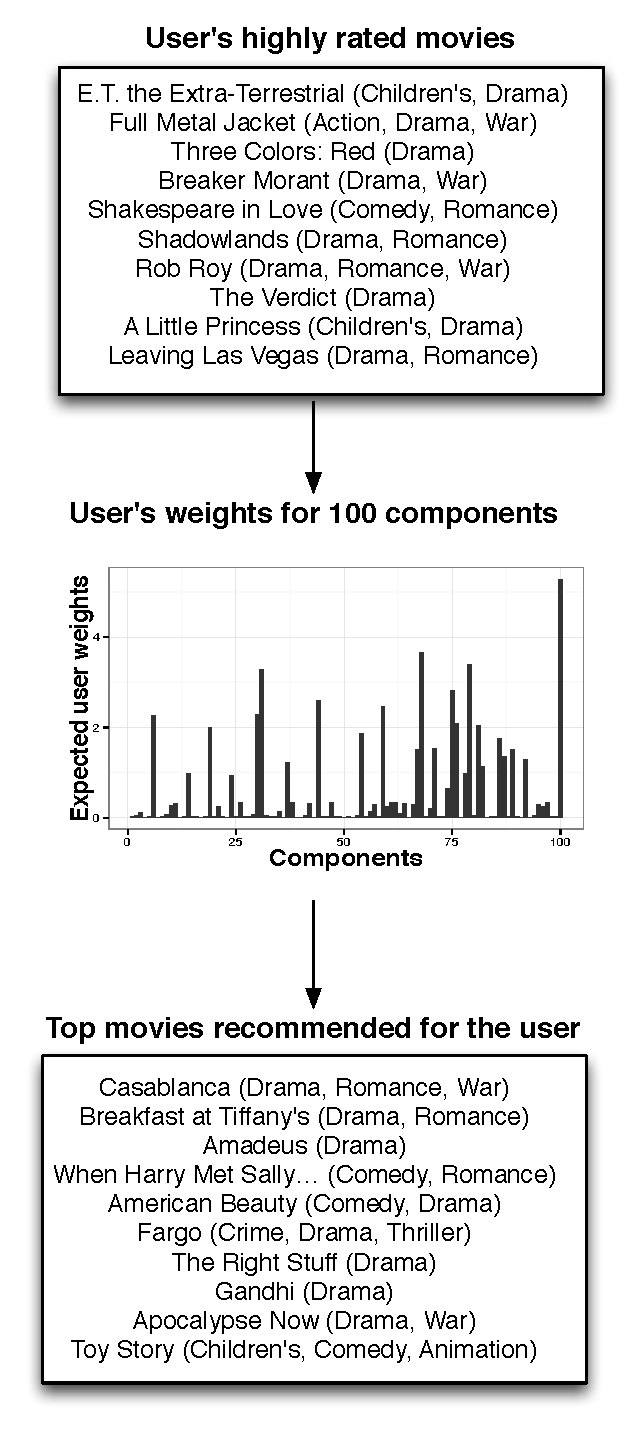
\includegraphics[width=0.5\columnwidth]{figures/movielens-user2.pdf}\\
\caption{An illustration showing a subset of the highly rated movies
  of a selected user $U$ in the MovieLens data set~\cite{Herlocker:1999},
  and a subset of the movies in the top 15 recommended to the user by
  our algorithm. The expected user's $K$-vector of weights $\theta_u$,
  inferred by our algorithm is shown. In our analysis, $K$ was set to
  100.}
\label{fig:movielens-illustration}
\end{figure}

However, the assumptions behind traditional MF are fundamentally
flawed when analyzing real-world user behavior data.  In real-world
data, each user has only rated a small subset of the large population
of available items. An item a user did \textit{not} rate can arise in
two ways: either she considered it and chose not to rate it or she did
not consider it at all.  Each user has a limited budget (of money,
attention, or time) and therefore most of the unrated items in the
matrix arise from users not considering (as opposed to actively disliking) them.

The issue with traditional MF is that it treats all the missing cells
as observations, as though every user has enough attention to consider
every available item and decide whether to rate it.  Thus, the missing
cells are seen as evidence for users not liking the items, and this
significantly biases the learned representations.  To address the
problem, researchers have patched MF in a variety of ways, for example
by artificially down-weighting the contribution of the unrated items~\cite{Hu:2008p9402},
by sub-sampling from the unrated items to give equal weight to the
rated items~\cite{Gantner:2012p9364,Dror:2012a}, or by explicitly modeling the unrated
items as missing data~\cite{Paquet:2013p9197}.

This issue is particularly critical when analyzing binary data, such
as product purchases or webpage clicks.  Binary behavior data records
whether each user consumed an item but does provide a rating.
Building recommendation systems from such matrices is known as
one-class collaborative filtering or recommendation with implicit
feedback~\cite{Hu:2008p9402,Paquet:2013p9197}.

In this paper, we develop a Bayesian Poisson factorization model as an
alternative to traditional MF for building recommendation systems.
Our model implicitly assumes that each user has a limited budget with
which to consume items~\cite{Goodhardt:1984}, and thus an item that a
user has consumed provides a stronger signal about her preferences
than an item that a user has not consumed.  With several kinds of data
sets---users rating movies~\cite{Herlocker:1999,Koren:2009}, users
listening to songs~\cite{Bertin-Mahieux:2011}, and users reading
scientific papers~\cite{Jack:2010}---we demonstrate that Poisson
factorization leads to better recommendations than both traditional
matrix factorization and its variants that adjust for sparse data.

Furthermore, Poisson factorization is computationally more efficient
than traditional MF.  Most algorithms for fitting MF must iterate over
all user/item pairs, which is expensive for even modestly-sized user
behavior matrices and cannot take advantage of the sparsity of the
data~\cite{Hu:2008p9402}.  (To address this issue, practical applications of matrix
factorization rely on stochastic optimization~\cite{Mairal:2010}.)  In
this paper, we derive efficient variational inference algorithms for
Poisson factorization that take advantage of the sparsity of the
data. Our algorithms need only iterate over the non-zero entries of
the user behavior matrix.  This lets us handle data at a scale that
basic (non-stochastic) MF algorithms cannot handle.



\begin{figure*}[t!]
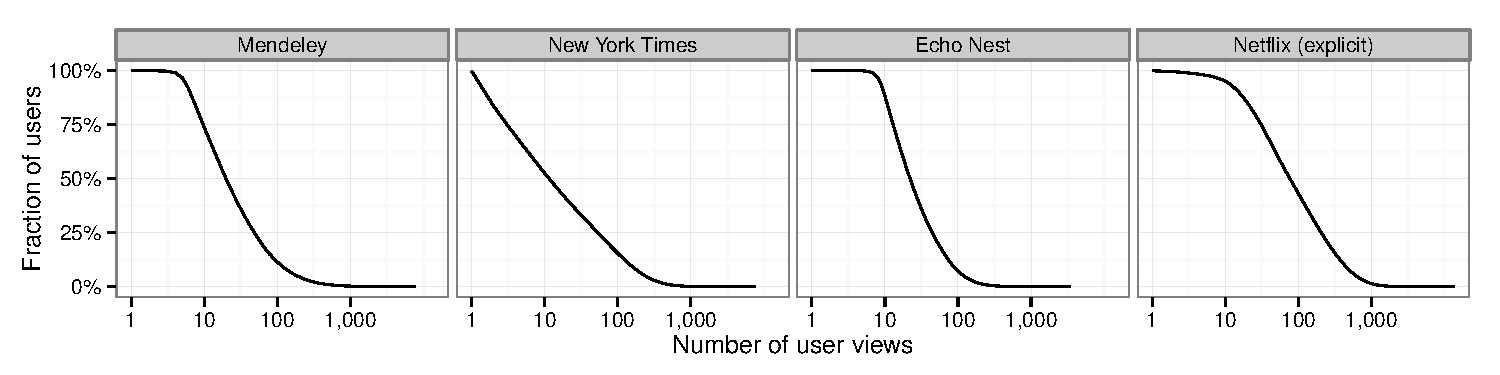
\includegraphics[width=\textwidth]{figures/user_activity_cdf.pdf}
\caption{Empirical complimentary cumulative distributions of user
  activity on each data set. Each curve shows the fraction of users
  who have consumed at least a given number of items. For instance,
  slightly less than half of all Netflix users have viewed at least
  100 movies.}
\label{fig:marginals}
\end{figure*}

%% \begin{figure*}[t!]
%% 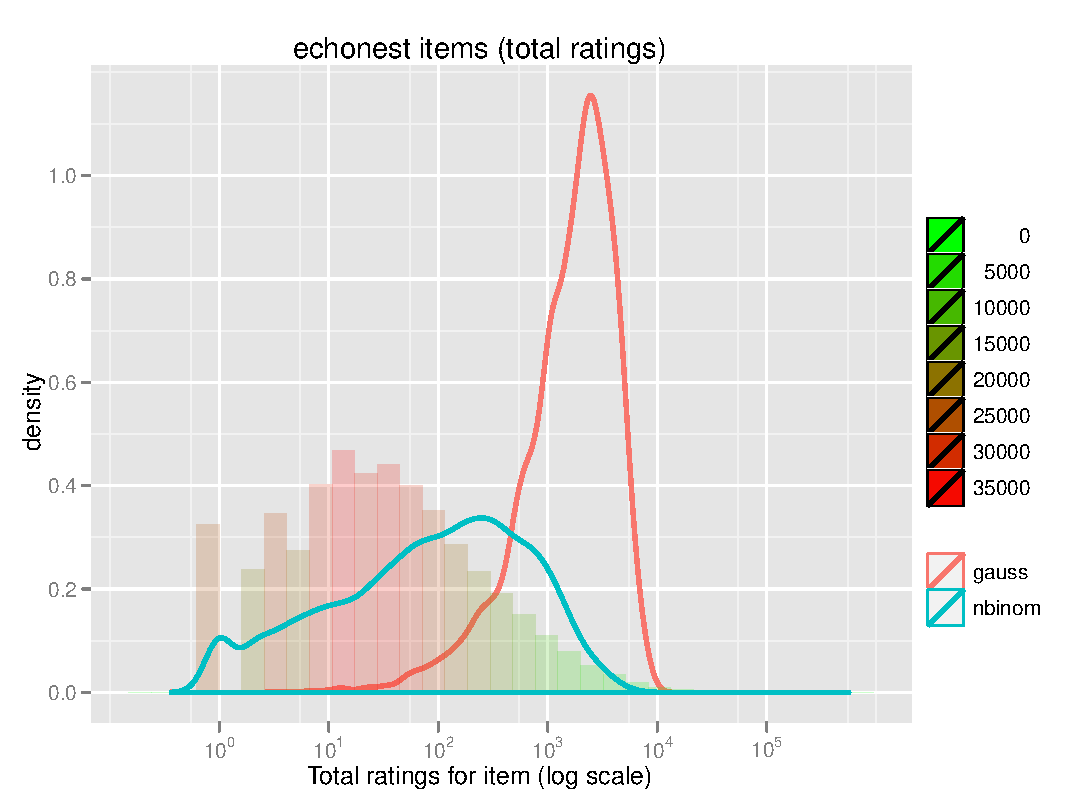
\includegraphics[width=0.33\textwidth]{figures/marginals/echonest.pdf}
%% 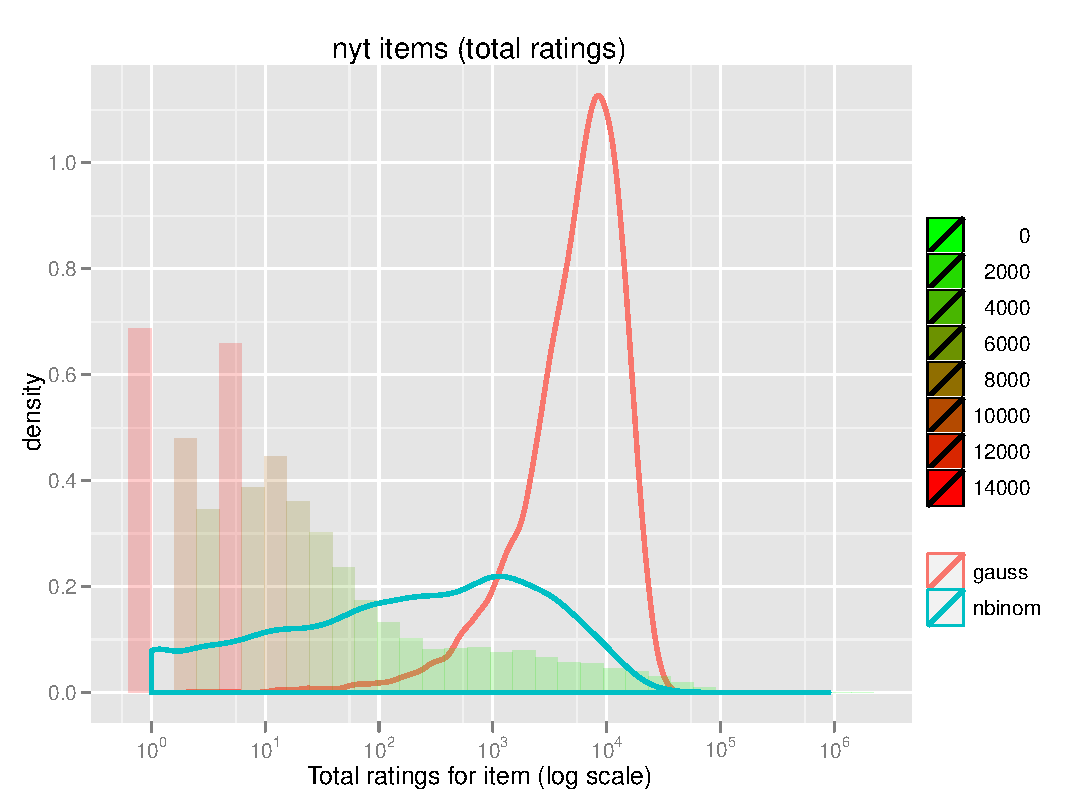
\includegraphics[width=0.33\textwidth]{figures/marginals/nyt.pdf}
%% 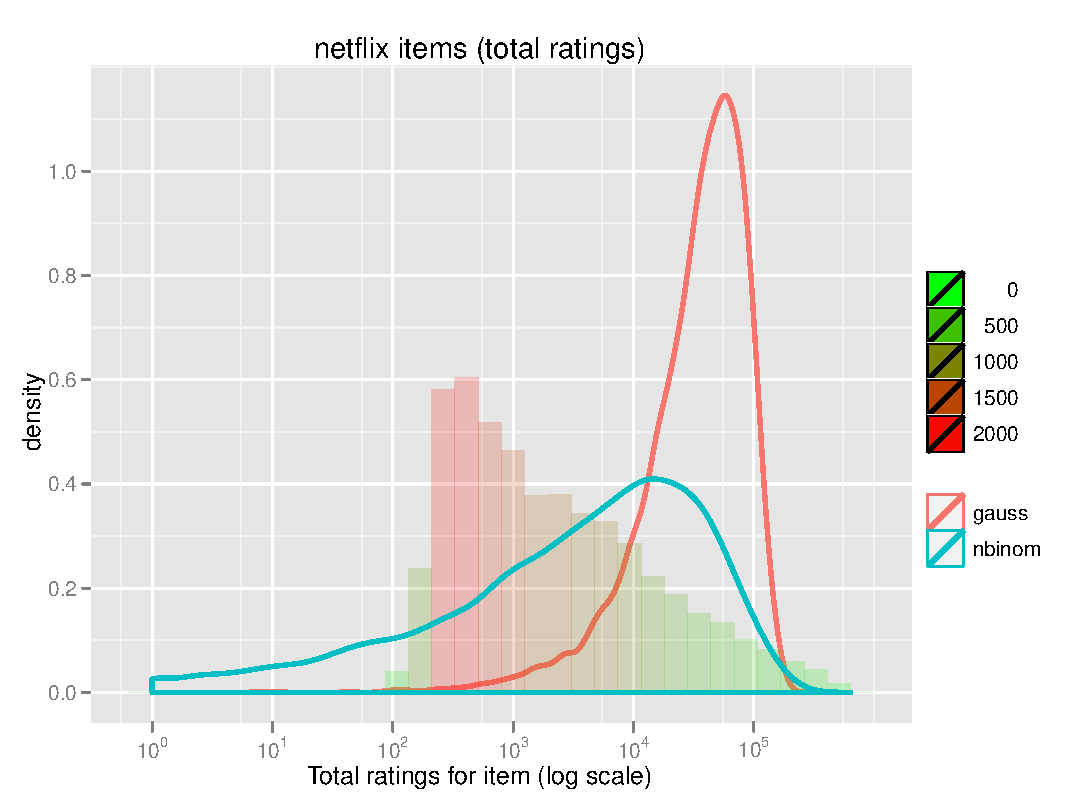
\includegraphics[width=0.33\textwidth]{figures/marginals/netflix.pdf}
%% \caption{Empirical distribution of item popularity on real datasets,
%%   with fitted negative binomial and Gaussian distributions. The
%%   distributions were fit using maximum likelihood estimation. The
%%   negative binomial places significant probability mass on the left
%%   tail, i.e., items with few ratings. The colored bars show that such
%%   items are the most frequent. In contrast, the Gaussian distribution
%%   places negligible mass on the left tail and mainly captures popular
%%   items. The mode of the negative binomial distribution is also closer
%%   to the empirical mode than the Gaussian distribution.}
%% \label{fig:marginals}
%% \end{figure*}

% prem: no longer use stochastic 

%% Further speed-ups using stochastic variational
%% inference~\cite{Hoffman:2013} let us fit Poisson factorization models
%% to massive data.

